% Part 5 chapter (file kept in part3/): one gauge across the device gauges of Part 3 and the cell gauges of Part 4.
% Values follow CANON/iam_canon.json (master table v1.1): per-cell H_min, M = E/k_BT = 20.94, one meaning for A. Symbols: Appendix~\ref{app:canon}.
\chapter{One gauge: the reading over its floor}\label{ch:onegauge}

\section*{The place}
IAM's Law (Chapter~\ref{ch:iams_law}): every irreversible transition from quantum superposition to classical record pays $k_BT\ln2$ per bit to
the nearest encoding surface, at that surface's temperature. A switching transistor, a measured qubit and a copied methylation mark are all
records written against thermal noise. The device gauges of Part~\ref{part:3} and the cell gauges of Part~\ref{part:4} read each of them the same
way: the measured record over the lowest record the system allows at its temperature. This chapter sets them on one gauge. Thermal noise is not
filtered out; it is the yardstick.

\section{The symbols}
\begin{center}\small\begin{tabular}{p{0.150\textwidth}p{0.300\textwidth}p{0.449\textwidth}}\toprule
symbol & meaning & in every domain\\\midrule
$A$ & reading $/$ healthy reference & dimensionless; $A=1$ is the system working as itself, the middle of the gauge\\
healthy reference & the denominator & the same system's healthy reading, on the same instrument\\
$H_{\min}$ & the floor & the lowest error the system can hold before thermal kicks win; below 1, nothing reads below it\\
$M$ & $E/k_BT$ & drive energy over the thermal noise quantum; $M/\ln2$ in Landauer units\\
$T$ & the temperature the record sees & the bath that writes on the record: the chip junction, the qubit's own mode, the cell; every floor is computed there\\\bottomrule
\end{tabular}\end{center}
Example of the energy scale: the AMD Ryzen 9 9950X (170\,W, $(20.0$--$20.6)\times10^9$ transistors, 4.3\,GHz~\cite{AMD9950X}, $T_j=75\,^\circ$C) switches at
$E_{\rm sw}=(1.92$--$1.97)\times10^{-18}$\,J, 576--593 times the Landauer floor, $M=399$--$411$; on its own gauge the Landauer floor therefore sits at 0.0017
(the transistor count, from die-level reports, is the least certain input)
(Chapter~\ref{ch:cmos}) \calc.

\paragraph{One gauge, each domain in its own form.} Every $A$ is an error score read on the same gauge (Fig.~\ref{fig:onegauge}): the reading
divided by the same system's healthy reading, so that $A=1$ is the system working as itself and sits in the middle. Below it lies $H_{\min}$, the
absolute lowest error the system can hold before thermal kicks win; nothing reads below $H_{\min}$. Above 1 the system makes more error than when
healthy. The formula is not the same in every domain, and should not be: the error comes from different physics in each (laser and motional noise in a
trapped ion, Rydberg decay in a neutral atom, two-level fluctuators in a transmon's oxides, a missed site at DNA
replication), and each field writes its thresholds in its own units.
\begin{center}\small\begin{tabular}{p{0.11\textwidth}p{0.24\textwidth}p{0.22\textwidth}p{0.29\textwidth}}\toprule
score & reading & healthy reference ($A=1$) & $H_{\min}$ (on the gauge)\\\midrule
IAM-A & copy error, $H(\varepsilon)$ & $P_{\rm cell}H(\varepsilon_0)$ & $H(\varepsilon_0)$; neutrophils at $1/P=0.910$\\
Met-A & $\langle H(\beta)\rangle$ at identity sites & purified healthy cells, same platform & an open problem for arrays\\
C-score & clustering of the residual map & healthy median clustering & ---\\
qubit gauge & $\varepsilon=-\ln(1-p_{2Q})$ & the device as built & thermal floor $p_{\rm eq}t_g/T_1$ (transmon reading: $6\times10^{-4}$)\\
chip gauge & $E_{\rm sw}=\mathrm{TDP}/(Nf)$ & the chip as built & Landauer floor $k_BT_j\ln2$ (9950X: $0.0017$)\\\bottomrule
\end{tabular}\end{center}
Some systems also have a point on the high side where they stop working: for a qubit, the gate error at which error correction fails ($p\approx1\,\%$;
the transmon worked example at $A=10$). For cells the high side is the cancer direction. Breach and the cancer region beyond it lie to the right of Normal and are to be measured on this scale from per-person data; the far end, a full
surface, is known: $1/0.330263=3.03$ on Met-A and $1/(P\,H(\varepsilon_0))=1/(1.099\times0.2043)=4.45$ on IAM-A for neutrophils ($H(\varepsilon_0)=0.2043$ bits at $\varepsilon_0=0.032$) \calc. For a compact star the far-right line is a
limiting mass: the Chandrasekhar mass for a white dwarf and the maximum (TOV) mass for a neutron star (Chapter~\ref{ch:blackholes}, Fig.~\ref{fig:stargauge}). The region between $H_{\min}$ and the healthy
band is less error than healthy; for cells what it means biologically is the next thing to measure.

\paragraph{The compartment, not the average.} A point of method carries over directly from the cell to the star. The cell instrument does
not score the whole person; it scores each cell type on its own. The star gauge does the same: it reads the core, not the whole star. A red
supergiant such as Betelgeuse is enormous and diffuse, so its overall structure looks unremarkable on any whole-body measure, exactly as a
person can look well while one cell type is in trouble. The signal is in the compartment, not the average. The supernova is a core event.
\analogy{} Stellar astrophysics already predicts these transitions with great precision by its own mature methods. The star gauge is not
offered as a new way to predict stars; it reproduces what astronomy already knows. Its purpose is to show that the cell and the star are
read by one instrument. The predictive novelty is on the biological side, where no such gauge existed before. \interp

\begin{figure}[htbp]\centering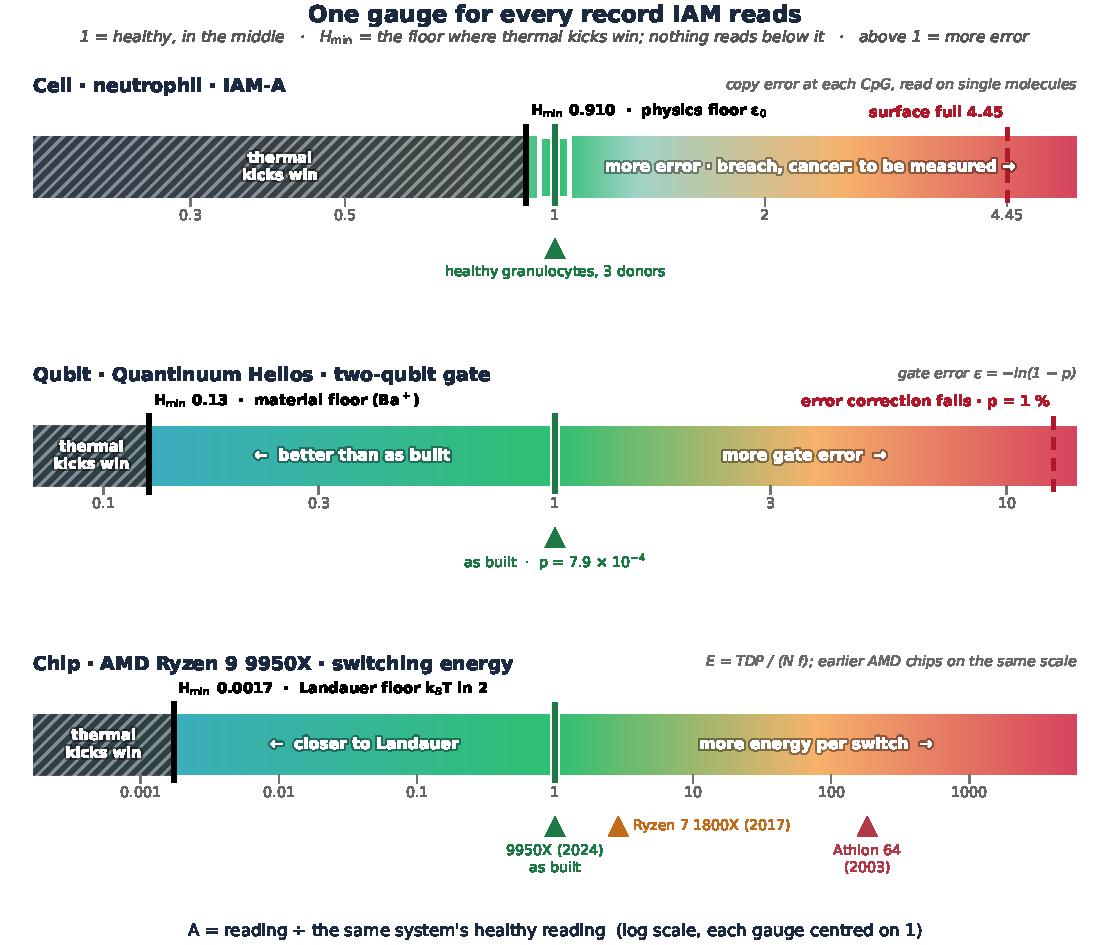
\includegraphics[width=\textwidth]{figures/part3/one_gauge.pdf}
\caption{One gauge for every score. $A=1$ is the healthy reading of that same system (green); $H_{\min}$ (grey line) is the lowest error it can hold
before thermal kicks win, and nothing reads below it (grey zone). Cell: neutrophil IAM-A (healthy granulocytes from three donors at 1), $H_{\min}=H(\varepsilon_0)$ at $1/P_{\rm cell}=0.910$, Normal
band 0.95--1.05; breach to be measured; surface full at 4.45. Qubit: a transmon at 5\,GHz and its own 35\,mK~\cite{Jin2015}, $T_1=68\,\mu$s~\cite{GoogleWillow2025}, an
illustrative 40\,ns gate and two-qubit error $10^{-3}$, against its thermal floor $p_{\rm eq}t_g/T_1=6.2\times10^{-7}$ (at $6.2\times10^{-4}$); error correction fails near
$p=1\,\%$. Chip: AMD Ryzen 9 9950X (170\,W, $(20.0$--$20.6)\times10^9$ transistors, 4.3\,GHz, $T_j=75\,^\circ$C) against the Landauer floor.
Each row has its own log scale, centred on 1.}\label{fig:onegauge}\end{figure}

\paragraph{Where $H_{\min}$ comes from.} For the cell, the form of the floor is IAM's Law: a holding energy $E_{\rm hold}$ against $k_BT$ allows
an error $\varepsilon_0=1/(1+e^{E_{\rm hold}/k_BT})$. Its height is at present measured: $E_{\rm hold}=\varphi M=3.41\,k_BT$ is read from the cells' own
copy error, read on the sorted-cell sequencing of the methylation atlas~\cite{Loyfer2023} (Chapter~\ref{ch:iama}), so $\varepsilon_0=0.032$ is the measured error expressed through the Boltzmann form, as a thermometer whose zero was set by a measurement
rather than by absolute zero. Three routes would make it absolute: the copying enzyme's own discrimination energy, $k_BT\ln(\text{selectivity})$ of
DNMT1 measured precisely in vitro (published values bracket $1.9$--$4.4\,k_BT$~\cite{Pradhan1999,Goyal2006,Adam2023}); a derivation of $\varphi$, the fraction of one ATP spent per held bit,
from the maintenance chemistry, since $M=20.94$ is already set by ATP; and the temperature test in ectotherms, where a fixed holding energy predicts a
different error at 10\,$^\circ$C than at 37\,$^\circ$C. That test is the next step: the fish read so far (Section~\ref{sec:og_temperature})
tracked a library-quality term, and the copy error depends on the read pipeline, so the test needs one species at two recorded temperatures on one
pipeline \openprob. For the
chip, $H_{\min}$ is the law itself. For the qubit it is the same law at the temperature the qubit itself sees: the occupation
$1/(1+e^{hf/\kB T})$ of the wrong level, with the same form as the cell's $\varepsilon_0$, and per gate $p_{\rm eq}t_g/T_1$
(Chapter~\ref{ch:qplatforms}) \derived.

\section{A is an error measurement}
At an identity site where the cell's pattern is methylated, a fraction $\varepsilon$ of the cell's DNA copies have lost the mark, so
$\beta=1-\varepsilon$; at an unmethylated identity site a fraction $\varepsilon$ have gained one, $\beta=\varepsilon$. Since
$H(\beta)=H(1-\beta)$, the entropy at either site is the entropy of the error:
\begin{equation}H(\beta)=H(\varepsilon),\qquad H(x)=-x\log_2x-(1-x)\log_2(1-x).\end{equation}
\paragraph{Met-A} (arrays) is the mean of $H(\beta)$ over the cell's identity sites divided by the same quantity on purified healthy cells of the
same type on the same platform, calibrated by the chain's own Stage~1:
\begin{equation}\text{Met-A}=\frac{\langle H(\beta)\rangle_{\rm identity\ sites}}{\langle H(\beta)\rangle_{\rm healthy\ reference}}.\end{equation}
Identity sites: across-array SD $\le0.05$; $\beta$ in $0.75$--$0.95$ or $0.05$--$0.25$; at most 3,000 per channel, and enough of them
measured. Neutrophils on EPIC v1: healthy reference $0.330263$ bits, from 6 purified healthy arrays (held-out SD $0.020$). In whole blood the denominator is
the healthy expectation for that person's own composition, $\langle H(\sum_c f_c\mu_{c,i})\rangle_i$, from their own cell fractions $f_c$ and
purified healthy profiles $\mu_c$; no cohort enters. The reading is made when neutrophils are above the read line.
\paragraph{The tare.} Every Met-A is read against healthy specimens run the same way (same slide, else same batch):
$A_{\rm rel}=A/\mathrm{median}(A_{\rm ref})$; nothing is fitted. The array's own noise index $N$, the mean $H(\beta)$ over the sites every
blood cell holds fixed, is checked against the references' range, and if it falls outside, the gauge state is withheld. The gauge is read on
$A_{\rm rel}$, and each reading states the smallest loss of the cell's pattern that specimen could have shown.
\paragraph{IAM-A} (single molecules) reads the copy error directly: $\varepsilon$ is the rate of an isolated unmethylated call between two
methylated calls, on molecules with at least 6 CpGs and at least 80\,\% methylated, on the methylated channel only. $P_{\rm cell}$ is valid only for the read-level pipeline it was measured on; a different pipeline needs its own healthy measurement first.
\begin{equation}\text{IAM-A}=\frac{H(\varepsilon)}{P_{\rm cell}\,H(\varepsilon_0)},\qquad \varepsilon_0=\frac{1}{1+e^{\varphi M}}=0.032,\end{equation}
with $M=20.94$, $\varphi=0.1628$ and $P_{\rm cell}$ the healthy cell's frozen position on the physics floor (neutrophils $1.099$).
\begin{itemize}
\item $A=1$: errors at the rate the healthy cell carries; Normal is $0.95$--$1.05$.
\item $A>1$: more error; the pattern is blurring.
\item $A<1$: less error than the standard; the pattern is locking tighter than normal.
\end{itemize}
Each reading has a C-score (built for Met-A, its healthy band being set next; the IAM-A C-score is defined and is the next to build): the clustering of the person's residual map along the genome, over the healthy baseline, so healthy reads 1 on the same
gauge. $A$ says how much error there is; the C-score says whether it is spread out or concentrated in regions.

The commissioned cell is the neutrophil. Other cells are added one at a time after passing the same tests.

\section{Two error channels}

\begin{figure}[htbp]\centering
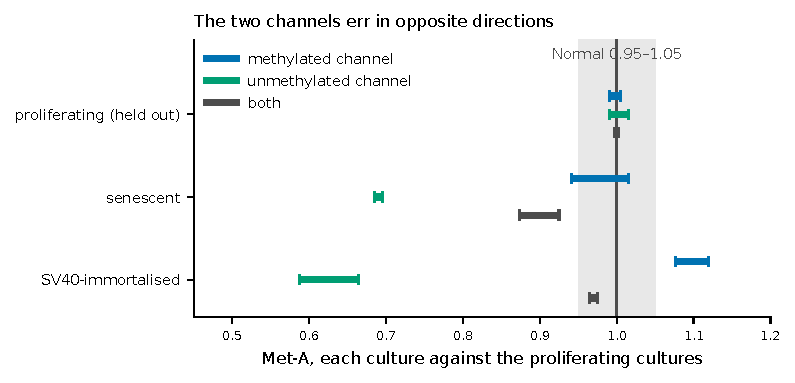
\includegraphics[width=0.8\textwidth]{figures/part3/fig_imr90_channels.pdf}
\caption{Met-A ranges per channel for IMR90 lung fibroblasts (WGBS, GSE48580), each culture read against the proliferating cultures. Senescent cultures hold the methylated channel near 1 and clean the unmethylated channel (0.685--0.695); SV40-immortalised cultures carry more error on the methylated channel (1.078--1.120) and less on the unmethylated one (0.587--0.664), and the combined reading (0.965--0.975) hides both. Grey: Normal, 0.95--1.05. \measured}\label{fig:imr90_channels}
\end{figure}
Methylated and unmethylated identity sites can err in opposite directions at once, so $A$ is reported per channel. IMR90 lung fibroblasts (WGBS, GSE48580~\cite{Cruickshanks2013}), each culture read against
the proliferating cultures, with sites chosen on one proliferating culture and the reference taken from another:
\begin{center}\small\begin{tabular}{lccc}\toprule
IMR90 & methylated channel & unmethylated channel & both\\\midrule
proliferating (held out) & 0.991--1.005 & 0.991--1.016 & 0.997--1.002\\
senescent & 0.941--1.016 & 0.685--0.695 & 0.874--0.925\\
SV40-immortalised & 1.078--1.120 & 0.587--0.664 & 0.965--0.975\\\bottomrule
\end{tabular}\end{center}
Senescent cells hold the methylated channel at the healthy rate and clean the unmethylated channel. Immortalised cells carry more error on the
methylated channel and less on the unmethylated one; the two cancel, and the reading over both channels sits inside Normal. Channels are
reported apart.

\section{The cell as a quantum computer}
\analogy\ The correspondence below is a vocabulary, not an identity of mechanism.
\begin{center}\small\begin{tabular}{p{0.240\textwidth}p{0.330\textwidth}p{0.330\textwidth}}\toprule
quantum computer & cell & what is measured\\\midrule
bit & one CpG site on one DNA copy & methylated or not\\
intended state & the cell's identity pattern & the cell's own standard\\
gate error (a write goes wrong) & copy error at division (DNMT1 misses a site) & isolated mismatches on single reads\\
$T_1$ decay (a stored bit relaxes) & erasure between divisions & region-wide loss, slow drift with age\\
leakage / crosstalk & de novo writing where it should not & coherent gains, often at CpG islands\\
error correction & neighbouring sites agreeing & neighbour agreement on single reads\\
error rate against specification & $A$ & $A$ per channel\\\bottomrule
\end{tabular}\end{center}
One caution. The array gauge measures \emph{state} error: the fraction of copies holding the wrong mark at one moment, which is what gate errors and
decay leave behind together. $A$ says how much error there is; read-level data say which channel produced it.

\section{What thermodynamics adds}

\begin{figure}[htbp]\centering
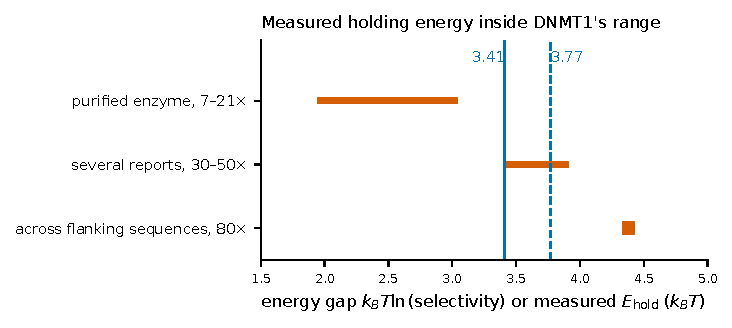
\includegraphics[width=0.62\textwidth]{figures/part3/fig_holding_energy.pdf}
\caption{Hopfield's energy gap $k_BT\ln({\rm selectivity})$ for the published in-vitro preferences of DNMT1 for hemimethylated CpG (7--21$\times$, about 30--40$\times$, 80$\times$~\cite{Pradhan1999,Goyal2006,Adam2023}): 1.9--4.4\,$k_BT$ \observed. Lines: the holding energy measured from the cells' copy error, 3.41\,$k_BT$ (copy channel, uncorrected) and 3.77\,$k_BT$ (instrument error removed) \measured. A consistency check: the published range is tenfold.}\label{fig:holding_energy}
\end{figure}
Met-A and IAM-A both measure in bits. Only IAM-A prices those bits against thermal noise, and that adds three things a reference standard
cannot give.
\paragraph{A physical floor.} $\varepsilon_0=1/(1+e^{\varphi M})$ comes from the energy budget, not from a reference population.
\paragraph{The holding energy in the law's units.} The measured copy error gives the energy the cell spends holding one methylation bit,
$E_{\rm hold}/k_BT=\ln[(1-\varepsilon)/\varepsilon]=3.41$, which is $4.9$ Landauer units ($k_BT\ln2$). One ATP is $\Delta G_{\rm ATP}/RT=
54{,}000/(8.314\times310.15)=20.94\,k_BT$ (this is $M$), or $30.2$ Landauer units. The cell spends $\varphi=3.41/20.94=0.163$ of one ATP per held
bit, the same in either unit.
\paragraph{A match to the copying enzyme.} Hopfield's relation (1974~\cite{Hopfield1974}): an enzyme that discriminates right from wrong with an energy gap $\Delta E$
errs at about $e^{-\Delta E/k_BT}$, so $\Delta E=k_BT\ln(\text{selectivity})$. Published in-vitro preferences of DNMT1 for hemimethylated over
unmethylated CpG: $7$--$21\times$ (purified recombinant enzyme~\cite{Pradhan1999}), about $30$--$40\times$ on short substrates~\cite{Goyal2006}, and $80\times$ on average across
flanking sequences~\cite{Adam2023}:
$\Delta E=\ln7$ to $\ln80=1.9$--$4.4\,k_BT$ \observed. The measured holding energy, $3.41\,k_BT$ (copy channel, uncorrected) and $3.77\,k_BT$ (instrument error
removed), lies inside that range. This is a consistency check, not a confirmation: the published range is tenfold, the selectivity maps most
directly onto the de novo channel, and UHRF1~\cite{Bostick2007,Sharif2007}, DNMT3 and TET also act in the cell.
\paragraph{Temperature.}\label{sec:og_temperature} IAM's Law prices a bit at the local temperature, so ectotherms are the natural test. So far: Methow steelhead red blood
cells at about $10\,^\circ$C read $3.31\,k_BT$, the same as human cells at $37\,^\circ$C ($3.29$--$3.51\,k_BT$); brook charr sperm $3.82$, Methow
sperm $4.02$, Atlantic salmon fin $3.47$, coho smolts $3.30\,k_BT$ (Chapter~\ref{ch:salmonid}). The pre-registered Methow temperature prediction was not met, and in every fish set the reading
also tracked a library-quality term (conversion failure or duplicates). No fish-level temperature effect can be read until that term is removed.

\section{Where the law enters, and where it does not}
The law enters through the cost per bit at the local temperature and through $M$. The virial half (Chapter~\ref{ch:virial_law}) holds inside every
molecule of a cell, as in every $1/r$-bound system (Chapter~\ref{ch:ledgers}), but the gauge does not use it: the reading needs only the cost per bit and
$M$. In each domain the gauge asks one question, how far the record sits above its floor, and states which quantities are measured (the reading,
$T$, $M$, the cell's holding energy) and which follow from $\kB T$ alone (the chip's Landauer floor and the qubit's thermal floor). Chapter~\ref{ch:reach} says what each gauge could give.

One gauge now reads a qubit, a processor and a cell on the same terms. A device physicist, a chip engineer and a geneticist can each read their own system on it and set their readings side by side.
